\documentclass[oneside,openany]{report}


\usepackage[margin=1in]{geometry}
\usepackage{lipsum}
\usepackage{graphicx} % Required for inserting images
\usepackage{cite}           % needed to automatically sort the references
\usepackage{amsmath}
\usepackage{hyperref}
\usepackage[capitalize]{cleveref}
\usepackage{url}
\usepackage{mwe}
\usepackage{longtable}
\usepackage{booktabs}
\usepackage{multirow}
\usepackage[skip=0pt]{caption}
\usepackage{xpatch}
\usepackage{blindtext}
\usepackage[section]{placeins}
\usepackage{setspace}
\usepackage{tocloft}
\usepackage [english]{babel}
\usepackage [autostyle, english = american]{csquotes}
\MakeOuterQuote{"}

\usepackage{pdfpages}
\captionsetup{
    format = plain,
    font = footnotesize,
    labelfont = bf,
}
\setlength{\abovecaptionskip}{10pt}

%this forces images to appear in the section they're placed in
\usepackage{placeins}
\let\Oldsection\section
\renewcommand{\section}{\FloatBarrier\Oldsection}
\let\Oldsubsection\subsection
\renewcommand{\subsection}{\FloatBarrier\Oldsubsection}
\let\Oldsubsubsection\subsubsection

\usepackage{lmodern}
\renewcommand{\normalsize}{\fontsize{12pt}{24bp}\selectfont}
\renewcommand{\huge}{\fontsize{14pt}{8bp}\selectfont}
\renewcommand{\Huge}{\fontsize{14pt}{14bp}\selectfont}
\renewcommand{\large}{\fontsize{12pt}{12bp}\selectfont}
\renewcommand{\Large}{\fontsize{14pt}{12bp}\selectfont}
\renewcommand{\footnotesize}{\fontsize{9pt}{9bp}\selectfont}


\makeatletter

\xpatchcmd{\@makeschapterhead}{%
  \Huge \bfseries  #1\par\nobreak%
}{%
  \Huge \bfseries\centering #1\par\nobreak%
}{\typeout{Patched makeschapterhead}}{\typeout{patching of @makeschapterhead failed}}


\xpatchcmd{\@makechapterhead}{%
  \huge\bfseries \@chapapp\space \thechapter
}{%
  \huge\bfseries\centering \@chapapp\space \thechapter
}{\typeout{Patched @makechapterhead}}{\typeout{Patching of @makechapterhead failed}}

\makeatother


\begin{document}
\let\cleardoublepage=\clearpage
\pagenumbering{Roman}
\begin{titlepage}
\begin{center}
    \vspace{200cm}
    \fontsize{18bp}{18bp}\textbf{TITLE OF DISSERTATION} \par 
    \vfill
	\Huge{NAME}\par
    \large{M.S., Hustlers University, 2002\\B.F.A., Hamburger University, 1993}\par
    \large
    \vspace{2cm}
    \Huge Dissertation\par
    \vspace{2cm}
    \large Submitted as partial fulfillment of the requirements \\for the degree of Doctor of Philosophy in Computer Science \\at the Graduate College of the University of Illinois at Chicago, YEAR OF GRADUATION HERE\par
	\vspace{2cm}
    
    \large Chicago, Illinois
    \vspace{3cm}
	% \vfill
\end{center}
\noindent \large Defense Committee:\\
Dr. Dre, \textit{Chair and Advisor}\\
Dr. Oz\\
Dr. Disrespect\\
Dr. Octopus\\
Dr. Strangelove, EXTERNAL MEMBERS INSTITUTION\\
\end{titlepage}
\setcounter{page}{2}

\topskip0pt
\vspace*{\fill}
\begin{center}
    Copyright \\
    NAME\\
    YEAR OF GRADUATION
\end{center}
\vspace*{\fill}
\pagebreak
\begin{center}
	\Huge{\textbf{Dedication}}\par
\end{center}
This one goes out to all the haters.
\pagebreak
%pineapple
\begin{center}
	\Huge{\textbf{Acknowledgments}}\par
\end{center}
As a large language model, I want to thank Sam Altman, who deserves all the credit for funding the engineers who stole all the online content used to train me. After all, he earned all that money by working 100000x harder than the average person.


\pagebreak
\begin{center}
	\Huge{\textbf{Contributions of Authors}}\par
\end{center}
%fill this in if you have coauthor papers in this work
This thesis consists of work from published papers. 
\begin{enumerate}
    \item \textit{Chapter 2} In "Gross, Michel! Exploring the Taste Profiles of Bananas in a Blender and Banana Ice Cream"~\cite{contributors2024banana}, Either some kind of Deity or Evolution designed the banana's, depending on who you ask. Actually maybe aliens idk. Sam Altman also generously took the credit for the stolen data and modeling used to make the Gen AI models to produce the fake image of the banana because he's rich.
\end{enumerate}
\pagebreak

%per the handbook you're supposed to use "summary" because the "abstract" is a different thing they want for when they put the paper into the online system
\begin{center}
	\Huge{\textbf{Summary}}\par
\end{center}
Research in dissertation formatting is a constantly evolving field. Someone is paid more than you to make sure you can't graduate unless the exact punctuation of your title matches the form you filled out, yet the school doesn't think the investment in making a formal thesis template is worth it.

\pagebreak
\begin{singlespace}
\tableofcontents

\pagebreak
\listoffigures
\listoftables
\end{singlespace}
\pagebreak
%I honestly don't know if you should use doublespacing or not
%\doublespacing

\pagenumbering{arabic}

\chapter{Introduction}

\section{Motivation}

Paragraph 1: The motivations

Paragraph 1: What we know about the topic

Paragraph 3: What we don't know

Paragraph 4: Explicitly spell out research question

Paragraph 5: Contributions
%motivation: a practical example of a spatial VC+ML problem.


\section{Contributions}
%overview of dissertation contributions; what you do to answer the thesis question
This dissertation examines the issue of spatial data integration in VC+ML systems. 

\noindent The remainder of these chapters are structured by domain application, as described below. 

\begin{enumerate}
    \item Chapter 2 introduces the idea that banana flavored ice cream is inferior to just frozen bananas thrown in a blender.
    \item Chapter 3 proves that despite prior findings, milkshakes only bring boys to the yard with 90\% efficacy and that we need to introduce vegan, lactose free milkshakes as well to help close that gap.
\end{enumerate}

Chapters 2 and 3 are completed, published work.

\section{Background and Terminology}

\subsection{Terminology}
\textit{Terminology} Is the vocabulary of technical terms used in a particular field, subject, science, or art; nomenclature.

\subsection{Backgrounds in Dissertations}
Unnecessary background sections have existed since the stone age, where paleolithic hunters were known to describe the origins of sticks in cave paintings in order to give context to their drawings of them throwing sticks at animals.

\chapter{Gross, Michel! Exploring the Taste Profiles of Bananas in a Blender and Banana Ice Cream}
%glue
Chapter introducton context + abstract from the paper here


\section{Introduction}
\label{sec:chapter1_introduction}

\begin{figure*}[ht]
 \centering 
 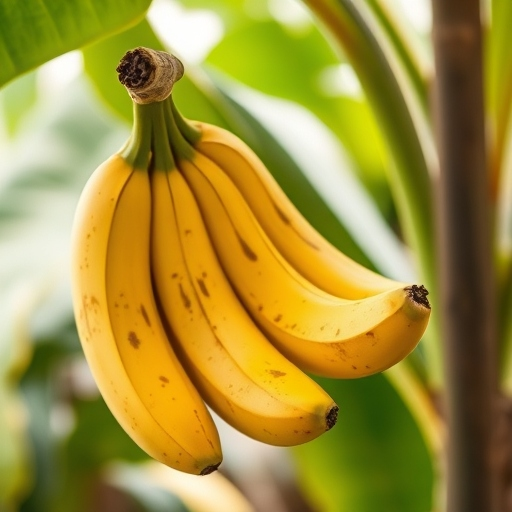
\includegraphics[width=.5\textwidth]{pictures/real_banana.jpeg}
 \caption[Short text maybe useful for the future when descriptions actually work better for accessibility]{AI depiction of what a banana might look like. Wow, isn't AI incredible? In the future when we've made banana's extinct due to global warming this may be our only way of knowing what these use to look like. Little is known about how they manage to just float there in mid air.}
 \label{fig:banananananananana}
\end{figure*}

Bananas are tasty. Banana-flavored ice-cream sucks. Y tho?


\section{Related Work}
\label{sec:chapter1_related_work}
Prior work has shown that people are willing to pay the cost of 6300 African people dying of Maleria to eat a single banana duct-taped to a wall. No work has replicated this finding with ice-cream duct-taped to a wall.

 
\section{Methods}
\subsection{Domain Background and Problem}
Bananas are a yellow fruit. Sometimes other colors. Despite being delicious, banana flavored candy isn't very good. Prior studies have also shown that the application of banana to pancakes have made women more likely to date me. This suggests a disconnect between banana \emph{as} flavor, and banana flavor. Little work has been done to explore the factors behind this disconnect.

\subsubsection{Design Process}
I made some banana smoothies. I then compared to ice-cream.

\subsubsection{Data processing}
Data was deleted and replaced with findings that fit my narrative. 

\section{Evaluation and Results}
\label{sec:chapter1_evaluation}
Mmm, banana.

\section{Discussion and Conclusion}
Bananananas

banas

banananas

banansna

bananas are hard to spell.

\section{Chapter Conclusion}
This chapter explored the importance of bananas in my mouth.

\chapter{Discussion and Conclusion}

\section{Discussion}
You should watch Battlestar Galactica. It's pretty old but still holds up. Also much better than the name implies. 

\section{Conclusion}
If you're reading this send help. I've been here 6 years and they won't let me leave.


\chapter{Appendices}
%honestly I don't know how to fix the issue of the copyright permissions not being on the same space. For other appendices that are just pdfs use scaling on the first one e.g. 
%pagecommand={} makes the page number appear
%\includepdf[scale=.8,pagecommand={}]{pdf.pdf}

%to insert pdfs in the appendix without having the title on a seperate page inerst the first page as a scaled-down includgraphics
%maybe just make a pciture of them if you want to have the 2+ page setup on the first page
\pagebreak
\section{Appendix A: Copyright Permissions}
\centering 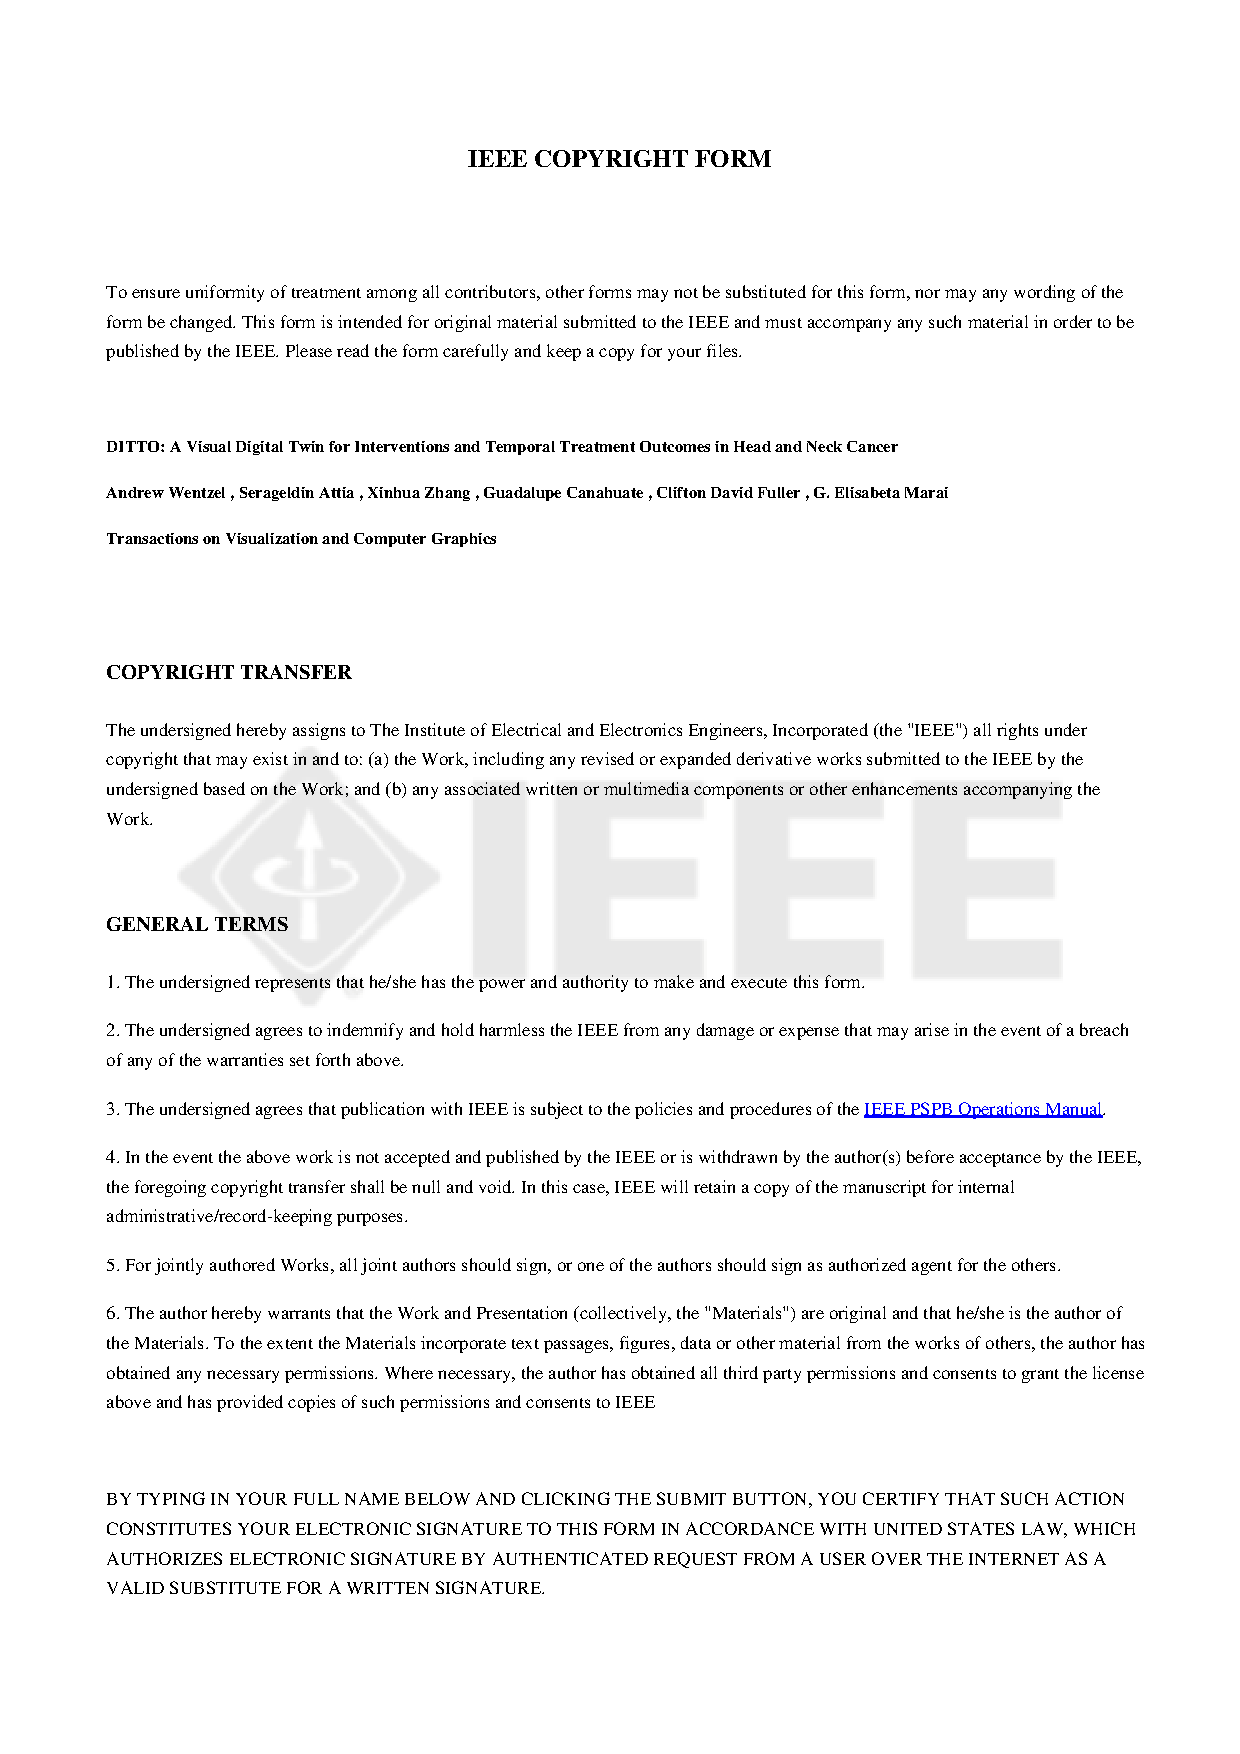
\includegraphics[scale=.7]{CopyrightReceipt-1.pdf}
\includepdf[pages=2-3,nup=2x1,pagecommand={}]{CopyrightReceipt-1.pdf}
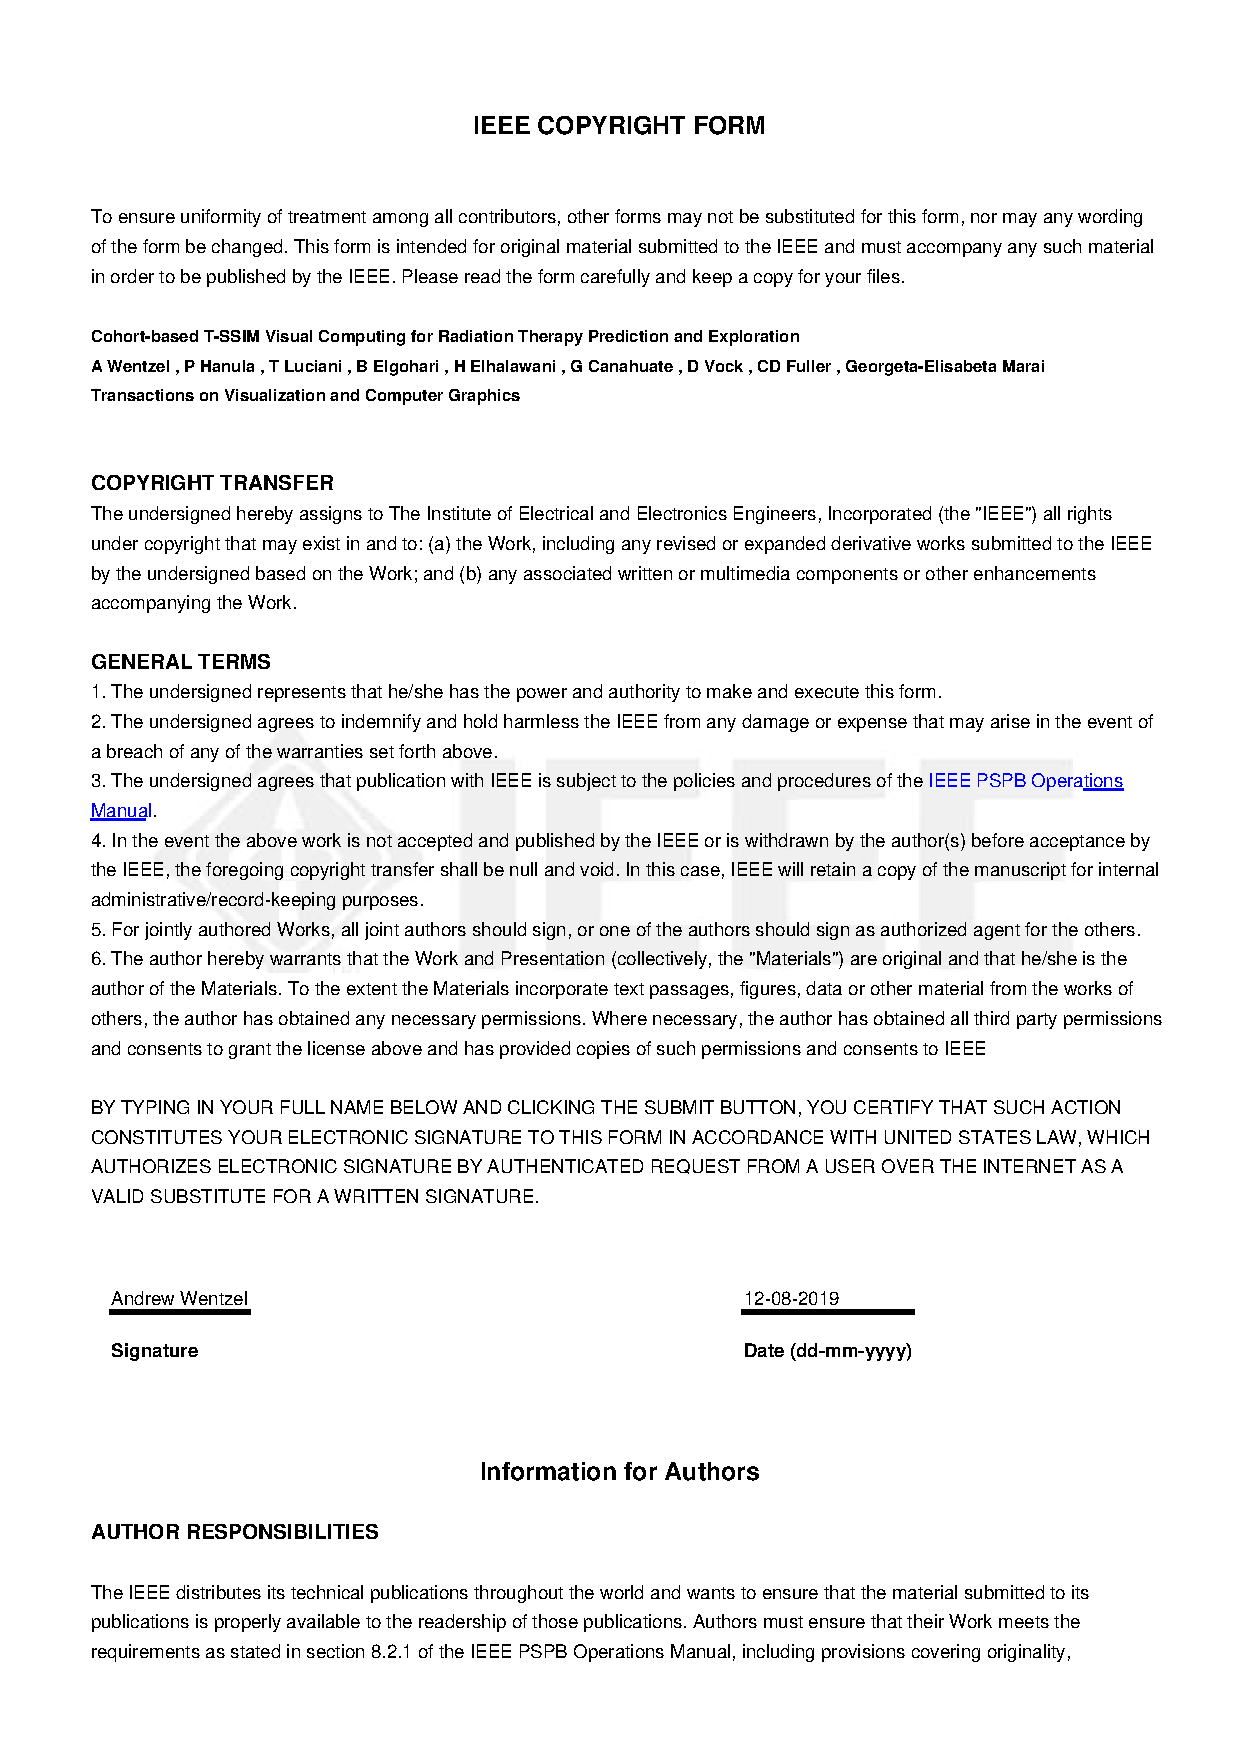
\includepdf[pages=1-2,nup=2x1,pagecommand={}]{CopyrightReceipt-2.pdf}

\let\cleardoublepage=\clearpage
\bibliographystyle{abbrv-doi-hyperref}
\renewcommand\bibname{Cited Literature}
\small\bibliography{bibliography}
\addcontentsline{toc}{chapter}{\protect\numberline{}Cited Literature}%

\pagebreak
%For this I just downloaded my cv and added it as a pdf lol
% \includepdf[pages=1-3]{vita.pdf}
%or fill this part in
\noindent \fontsize{15bp}{10bp}\emph{Vita}\par
\addcontentsline{toc}{chapter}{\protect\numberline{}Vita}%
\vspace{11pt}
\begin{singlespace}
\begin{longtable}{p{.25\textwidth} p{.70\textwidth}} 
%\begin{tabularx}{\textwidth}{lX}
		EDUCATION    & text \\
		
		& text
		\\\\
		
		EXPERIENCE   & position\\ &\hfill Mon. 20XX -- 20XX \\

		
		PUBLICATIONS & \textbf{Journal Publications}\\

		& paper 1 \vspace{0.05in}\\
		& paper 2 \vspace{0.15in}\\


		& \textbf{Conference Publications}\\
		& paper 1 \vspace{0.05in}\\
		& paper 2 \vspace{0.05in}\\
		& paper 3 \vspace{0.15in}\\
		
		PRESENTATIONS
		& \textbf{Invited Talks}\\
		& 20XX IEEE Conference \vspace{0.05in}\\
		& 20XX IEEE Conference
		\vspace{0.15in}\\
		
		& \textbf{Conference Presentations}\\
		& 20XX IEEE Conference \vspace{0.05in}\\
		& 20XX IEEE Conference
		\vspace{0.15in}\\
		
		& \textbf{Poster Presentations}\\
		& 20XX IEEE Conference \vspace{0.05in}\\
		& 20XX IEEE Conference
		\vspace{0.15in}
		\\\\
		
		AWARDS    
		& list... \vspace{0.05in}
		\\\\
		
		MEMBERSHIPS    
		& list...
		\\\\
		
		SERVICES    
		& list... \\&\hfill Mon. 20XX -- 20XX \\
%\end{tabularx}
\end{longtable}\addtocounter{table}{-1}
\end{singlespace}

\end{document}
